
\node [circle , draw] (zero) {0}; 
\path (zero) edge [loop below] (zero); 
\path (zero) edge [loop above] (zero);
\path (zero) edge [loop left] (zero); 
\path (zero) edge [loop right] (zero);

\begin{figure}[!hbt]
\centering
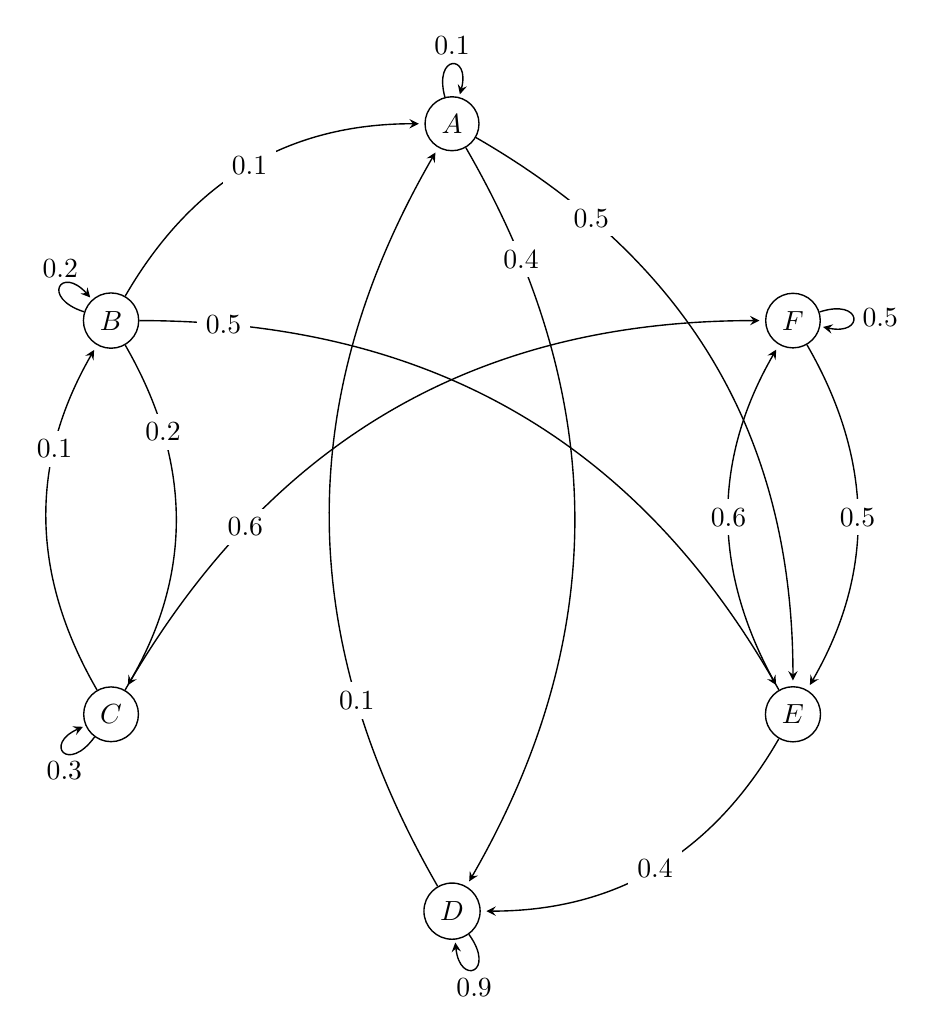
\begin{tikzpicture}[->,>=stealth,shorten >=2pt, line width=0.5pt, node distance=2cm]
% Nodos
\node [circle , draw] (A)  at  (90:5cm) {$A$};
\node [circle , draw] (B)  at (150:5cm) {$B$};
\node [circle , draw] (C)  at (210:5cm) {$C$};
\node [circle , draw] (D)  at (270:5cm) {$D$};
\node [circle , draw] (E)  at (330:5cm) {$E$};
\node [circle , draw] (F)  at  (30:5cm) {$F$};
% Ejes
% ---
% A
% ---
\path (A) edge [loop above] node [above] {$0.1$} (A);

%\path (A) edge [bend left] node [fill=white, anchor=center, pos=0.3] {$0.3$} (B);

%\path (A) edge [bend left] node [fill=white, anchor=center, pos=0.7] {$0.3$} (C);

\path (A) edge [bend left] node [fill=white, anchor=center, pos=0.15] {$0.4$} (D);

\path (A) edge [bend left] node [fill=white, anchor=center, pos=0.2] {$0.5$} (E);

%\path (A) edge [bend left] node [above right] {$0.5$} (F);

% ---
% B
% ---
\path (B) edge [in=132, out=162, loop] node [above] {$0.2$} (B);

\path (B) edge [bend left] node [fill=white, anchor=center, pos=0.5] {$0.1$} (A);

\path (B) edge [bend left] node [fill=white, anchor=center, pos=0.25] {$0.2$} (C);

%\path (B) edge [bend left] node [fill=white, anchor=center, pos=0.75] {$0.2$} (D);

\path (B) edge [bend left] node [fill=white, anchor=center, pos=0.1] {$0.5$} (E);

%\path (B) edge [bend left] node [fill=white, anchor=center, pos=0.7] {$0.5$} (F);
% ---
% C
% ---
\path (C) edge [in=204, out=234, loop] node [below] {$0.3$} (C);

%\path (C) edge [bend left] node [fill=white, anchor=center, pos=0.15] {$0.5$} (A);

\path (C) edge [bend left] node [fill=white, anchor=center, pos=0.7] {$0.1$} (B);

%\path (C) edge [bend left] node [right] {$0.0$} (D);

%\path (C) edge [bend left] node [above right] {$0.0$} (E);

\path (C) edge [bend left] node [fill=white, anchor=center, pos=0.25] {$0.6$} (F);
% ---
% D
% ---
\path (D) edge [in=276, out=306, loop] node [below] {$0.9$} (D);

\path (D) edge [bend left] node [fill=white, anchor=center, pos=0.25] {$0.1$} (A);

%\path (D) edge [bend left] node [fill=white, anchor=center, pos=0.25] {$0.5$} (B);

%\path (D) edge [bend left] node [right] {$0.0$} (C);

%\path (D) edge [bend left] node [above right] {$0.0$} (E);

%\path (D) edge [bend left] node [fill=white, anchor=center, pos=0.7] {$0.6$} (F);
% ---
% E
% ---
%\path (E) edge [in=348, out=18, loop] node [right] {$0.5$} (E);
%\path (E) edge [bend left] node [below] {$0.3$} (A);

%\path (E) edge [bend left] node [fill=white, anchor=center, pos=0.25] {$0.3$} (B);

%\path (E) edge [bend left] node [right] {$0.0$} (C);

\path (E) edge [bend left] node [fill=white, anchor=center, pos=0.5] {$0.4$} (D);

\path (E) edge [bend left] node [fill=white, anchor=center, pos=0.5] {$0.6$} (F);
% ---
% F
% ---
\path (F) edge [in=348, out=18, loop] node [right] {$0.5$} (F);
%\path (E) edge [bend left] node [below] {$0.3$} (A);

%\path (F) edge [bend left] node [fill=white, anchor=center, pos=0.25] {$0.3$} (B);

%\path (F) edge [bend left] node [right] {$0.0$} (C);

%\path (F) edge [bend left] node [fill=white, anchor=center, pos=0.5] {$0.4$} (D);

\path (F) edge [bend left] node [fill=white, anchor=center, pos=0.5] {$0.5$} (E);
\end{tikzpicture} 
\caption{Ejercicio 1b} 
\label{fig:1b}
\end{figure}








\begin{figure}[!hbt]
\centering
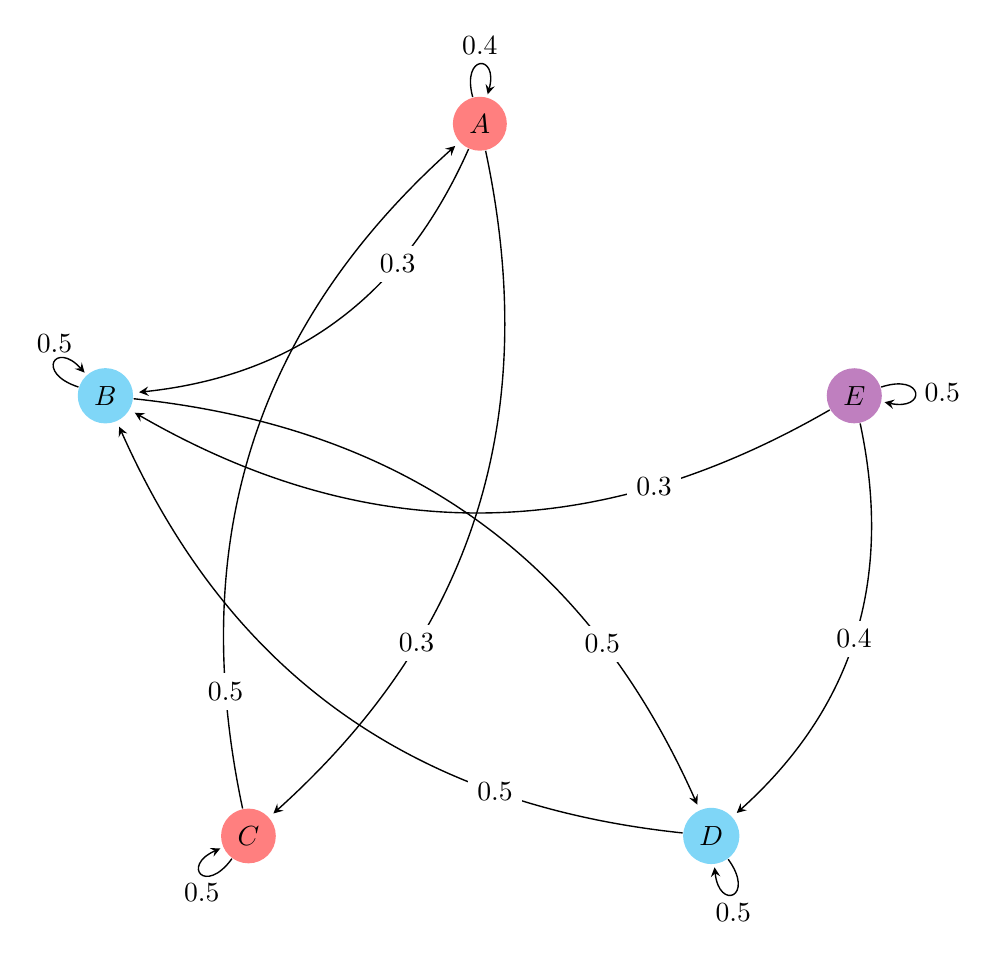
\begin{tikzpicture}[->, >=stealth,shorten >=2pt, line width=0.5pt, node distance=2cm]
% Nodos
\node [circle , fill=red, opacity=0.5,text opacity=1, text=black] (A)  at  (90:5cm) {$A$};
\node [circle , fill=cyan, opacity=0.5,text opacity=1, text=black] (B)  at (162:5cm) {$B$};
\node [circle , fill=red, opacity=0.5,text opacity=1, text=black] (C)  at (234:5cm) {$C$};
\node [circle , fill=cyan, opacity=0.5,text opacity=1, text=black] (D)  at (306:5cm) {$D$};
\node [circle , fill=violet, opacity=0.5,text opacity=1, text=black] (E)  at  (18:5cm) {$E$};
% Ejes
% ---
% A
% ---
\path (A) edge [loop above] node [above] {$0.4$} (A);

\path (A) edge [bend left] node [fill=white, anchor=center, pos=0.3] {$0.3$} (B);

\path (A) edge [bend left] node [fill=white, anchor=center, pos=0.7] {$0.3$} (C);

%\path (A) edge [bend left] node [right] {$0.0$} (D);

%\path (A) edge [bend left] node [above right] {$0.0$} (E);

% ---
% B
% ---
\path (B) edge [in=132, out=162, loop] node [above] {$0.5$} (B);

%\path (B) edge [bend left] node [below] {$0.3$} (A);

%\path (B) edge [bend left] node [right] {$0.3$} (C);

\path (B) edge [bend left] node [fill=white, anchor=center, pos=0.75] {$0.5$} (D);

%\path (B) edge [bend left] node [above right] {$0.0$} (E);
% ---
% C
% ---
\path (C) edge [in=204, out=234, loop] node [below] {$0.5$} (C);

\path (C) edge [bend left] node [fill=white, anchor=center, pos=0.15] {$0.5$} (A);

%\path (C) edge [bend left] node [right] {$0.3$} (B);

%\path (C) edge [bend left] node [right] {$0.0$} (D);

%\path (C) edge [bend left] node [above right] {$0.0$} (E);
% ---
% D
% ---
\path (D) edge [in=276, out=306, loop] node [below] {$0.5$} (D);

%\path (D) edge [bend left] node [below] {$0.3$} (A);

\path (D) edge [bend left] node [fill=white, anchor=center, pos=0.25] {$0.5$} (B);

%\path (D) edge [bend left] node [right] {$0.0$} (C);

%\path (D) edge [bend left] node [above right] {$0.0$} (E);
% ---
% E
% ---
\path (E) edge [in=348, out=18, loop] node [right] {$0.5$} (E);
%\path (E) edge [bend left] node [below] {$0.3$} (A);

\path (E) edge [bend left] node [fill=white, anchor=center, pos=0.25] {$0.3$} (B);

%\path (E) edge [bend left] node [right] {$0.0$} (C);

\path (E) edge [bend left] node [fill=white, anchor=center, pos=0.5] {$0.4$} (D);

  %\begin{pgfonlayer}{bg}
    %\draw[wrap=red, -](A.center)   to(B.center);
    %\draw[wrap=red](A0.center)   to[out=0,in=180](B2.center);
    %\draw[wrap=green](A1.center) to[out=0,in=180](B1.center);
    %\draw[wrap=green](A1.center) to[out=0,in=180](B3.center);
    %\draw[wrap=blue](A3.center)  to[out=0,in=180](B1.center);
  %\end{pgfonlayer}

\end{tikzpicture} 
\caption{Ejercicio 1a} 
\label{fig:1a}
\end{figure}
\newpage
\begin{figure}[!hbt]
\centering
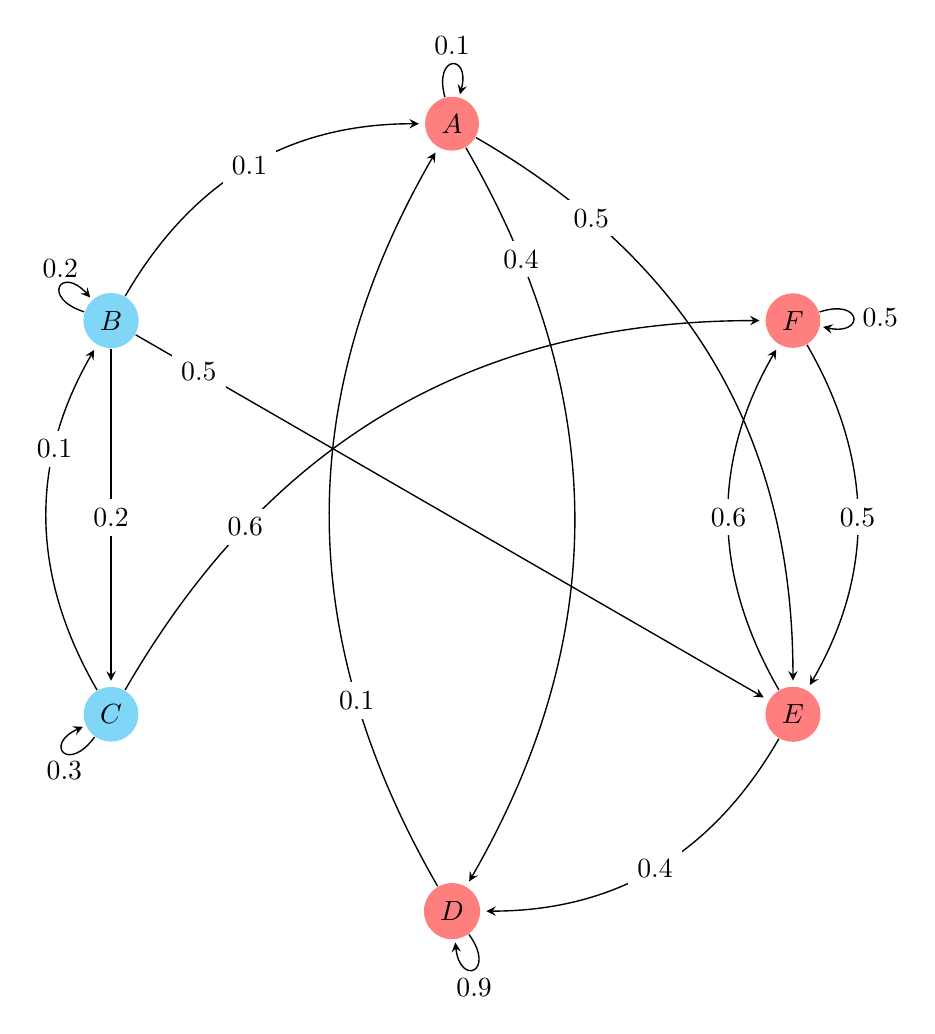
\begin{tikzpicture}[->,>=stealth,shorten >=2pt, line width=0.5pt, node distance=2cm]
% Nodos
\node [circle , fill=red, opacity=0.5,text opacity=1, text=black] (A)  at  (90:5cm) {$A$};
\node [circle , fill=cyan, opacity=0.5,text opacity=1, text=black] (B)  at (150:5cm) {$B$};
\node [circle , fill=cyan, opacity=0.5,text opacity=1, text=black] (C)  at (210:5cm) {$C$};
\node [circle , fill=red, opacity=0.5,text opacity=1, text=black] (D)  at (270:5cm) {$D$};
\node [circle , fill=red, opacity=0.5,text opacity=1, text=black] (E)  at (330:5cm) {$E$};
\node [circle , fill=red, opacity=0.5,text opacity=1, text=black] (F)  at  (30:5cm) {$F$};
% Ejes
% ---
% A
% ---
\path (A) edge [loop above] node [above] {$0.1$} (A);

%\path (A) edge [bend left] node [fill=white, anchor=center, pos=0.3] {$0.3$} (B);

%\path (A) edge [bend left] node [fill=white, anchor=center, pos=0.7] {$0.3$} (C);

\path (A) edge [bend left] node [fill=white, anchor=center, pos=0.15] {$0.4$} (D);

\path (A) edge [bend left] node [fill=white, anchor=center, pos=0.2] {$0.5$} (E);

%\path (A) edge [bend left] node [above right] {$0.5$} (F);

% ---
% B
% ---
\path (B) edge [in=132, out=162, loop] node [above] {$0.2$} (B);

\path (B) edge [bend left] node [fill=white, anchor=center, pos=0.5] {$0.1$} (A);

\path (B) edge [] node [fill=white, anchor=center, pos=0.5] {$0.2$} (C);

%\path (B) edge [bend left] node [fill=white, anchor=center, pos=0.75] {$0.2$} (D);

\path (B) edge [] node [fill=white, anchor=center, pos=0.1] {$0.5$} (E);

%\path (B) edge [bend left] node [fill=white, anchor=center, pos=0.7] {$0.5$} (F);
% ---
% C
% ---
\path (C) edge [in=204, out=234, loop] node [below] {$0.3$} (C);

%\path (C) edge [bend left] node [fill=white, anchor=center, pos=0.15] {$0.5$} (A);

\path (C) edge [bend left] node [fill=white, anchor=center, pos=0.7] {$0.1$} (B);

%\path (C) edge [bend left] node [right] {$0.0$} (D);

%\path (C) edge [bend left] node [above right] {$0.0$} (E);

\path (C) edge [bend left] node [fill=white, anchor=center, pos=0.25] {$0.6$} (F);
% ---
% D
% ---
\path (D) edge [in=276, out=306, loop] node [below] {$0.9$} (D);

\path (D) edge [bend left] node [fill=white, anchor=center, pos=0.25] {$0.1$} (A);

%\path (D) edge [bend left] node [fill=white, anchor=center, pos=0.25] {$0.5$} (B);

%\path (D) edge [bend left] node [right] {$0.0$} (C);

%\path (D) edge [bend left] node [above right] {$0.0$} (E);

%\path (D) edge [bend left] node [fill=white, anchor=center, pos=0.7] {$0.6$} (F);
% ---
% E
% ---
%\path (E) edge [in=348, out=18, loop] node [right] {$0.5$} (E);
%\path (E) edge [bend left] node [below] {$0.3$} (A);

%\path (E) edge [bend left] node [fill=white, anchor=center, pos=0.25] {$0.3$} (B);

%\path (E) edge [bend left] node [right] {$0.0$} (C);

\path (E) edge [bend left] node [fill=white, anchor=center, pos=0.5] {$0.4$} (D);

\path (E) edge [bend left] node [fill=white, anchor=center, pos=0.5] {$0.6$} (F);
% ---
% F
% ---
\path (F) edge [in=348, out=18, loop] node [right] {$0.5$} (F);
%\path (E) edge [bend left] node [below] {$0.3$} (A);

%\path (F) edge [bend left] node [fill=white, anchor=center, pos=0.25] {$0.3$} (B);

%\path (F) edge [bend left] node [right] {$0.0$} (C);

%\path (F) edge [bend left] node [fill=white, anchor=center, pos=0.5] {$0.4$} (D);

\path (F) edge [bend left] node [fill=white, anchor=center, pos=0.5] {$0.5$} (E);
\end{tikzpicture} 
\caption{Ejercicio 1b} 
\label{fig:1b}
\end{figure}
\begin{figure}[!hbt]
\centering
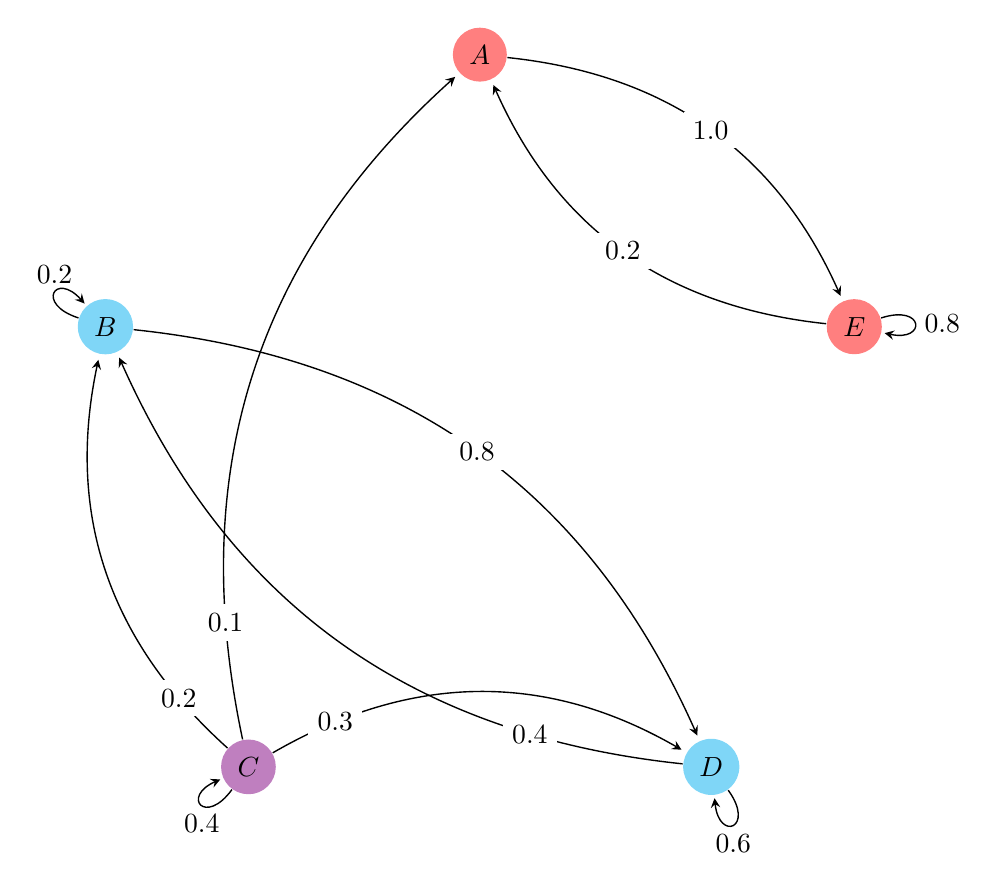
\begin{tikzpicture}[->,>=stealth,shorten >=2pt, line width=0.5pt, node distance=2cm]
% Nodos
\node [circle , fill=red, opacity=0.5,text opacity=1, text=black] (A)  at  (90:5cm) {$A$};
\node [circle , fill=cyan, opacity=0.5,text opacity=1, text=black] (B)  at (162:5cm) {$B$};
\node [circle , fill=violet, opacity=0.5,text opacity=1, text=black] (C)  at (234:5cm) {$C$};
\node [circle , fill=cyan, opacity=0.5,text opacity=1, text=black] (D)  at (306:5cm) {$D$};
\node [circle , fill=red, opacity=0.5,text opacity=1, text=black] (E)  at  (18:5cm) {$E$};
% Ejes
% ---
% A
% ---
%\path (A) edge [loop above] node [above] {$0.4$} (A);

%\path (A) edge [bend left] node [fill=white, anchor=center, pos=0.3] {$0.3$} (B);

%\path (A) edge [bend left] node [fill=white, anchor=center, pos=0.7] {$0.3$} (C);

%\path (A) edge [bend left] node [right] {$0.0$} (D);

\path (A) edge [bend left] node [fill=white, anchor=center, pos=0.5] {$1.0$} (E);

% ---
% B
% ---
\path (B) edge [in=132, out=162, loop] node [above] {$0.2$} (B);

%\path (B) edge [bend left] node [below] {$0.3$} (A);

%\path (B) edge [bend left] node [right] {$0.3$} (C);

\path (B) edge [bend left] node [fill=white, anchor=center, pos=0.5] {$0.8$} (D);

%\path (B) edge [bend left] node [above right] {$0.0$} (E);
% ---
% C
% ---
\path (C) edge [in=204, out=234, loop] node [below] {$0.4$} (C);

\path (C) edge [bend left] node [fill=white, anchor=center, pos=0.15] {$0.1$} (A);

\path (C) edge [bend left] node [fill=white, anchor=center, pos=0.15] {$0.2$} (B);

\path (C) edge [bend left] node [fill=white, anchor=center, pos=0.15] {$0.3$} (D);

%\path (C) edge [bend left] node [above right] {$0.0$} (E);
% ---
% D
% ---
\path (D) edge [in=276, out=306, loop] node [below] {$0.6$} (D);

%\path (D) edge [bend left] node [below] {$0.3$} (A);

\path (D) edge [bend left] node [fill=white, anchor=center, pos=0.2] {$0.4$} (B);

%\path (D) edge [bend left] node [right] {$0.0$} (C);

%\path (D) edge [bend left] node [above right] {$0.0$} (E);
% ---
% E
% ---
\path (E) edge [in=348, out=378, loop] node [right] {$0.8$} (E);
\path (E) edge [bend left] node [fill=white, anchor=center, pos=0.5] {$0.2$} (A);

%\path (E) edge [bend left] node [fill=white, anchor=center, pos=0.25] {$0.3$} (B);

%\path (E) edge [bend left] node [right] {$0.0$} (C);

%\path (E) edge [bend left] node [fill=white, anchor=center, pos=0.5] {$0.4$} (D);
\end{tikzpicture} 
\caption{Ejercicio 1c} 
\label{fig:1c}
\end{figure}
\begin{figure}[!hbt]
\centering
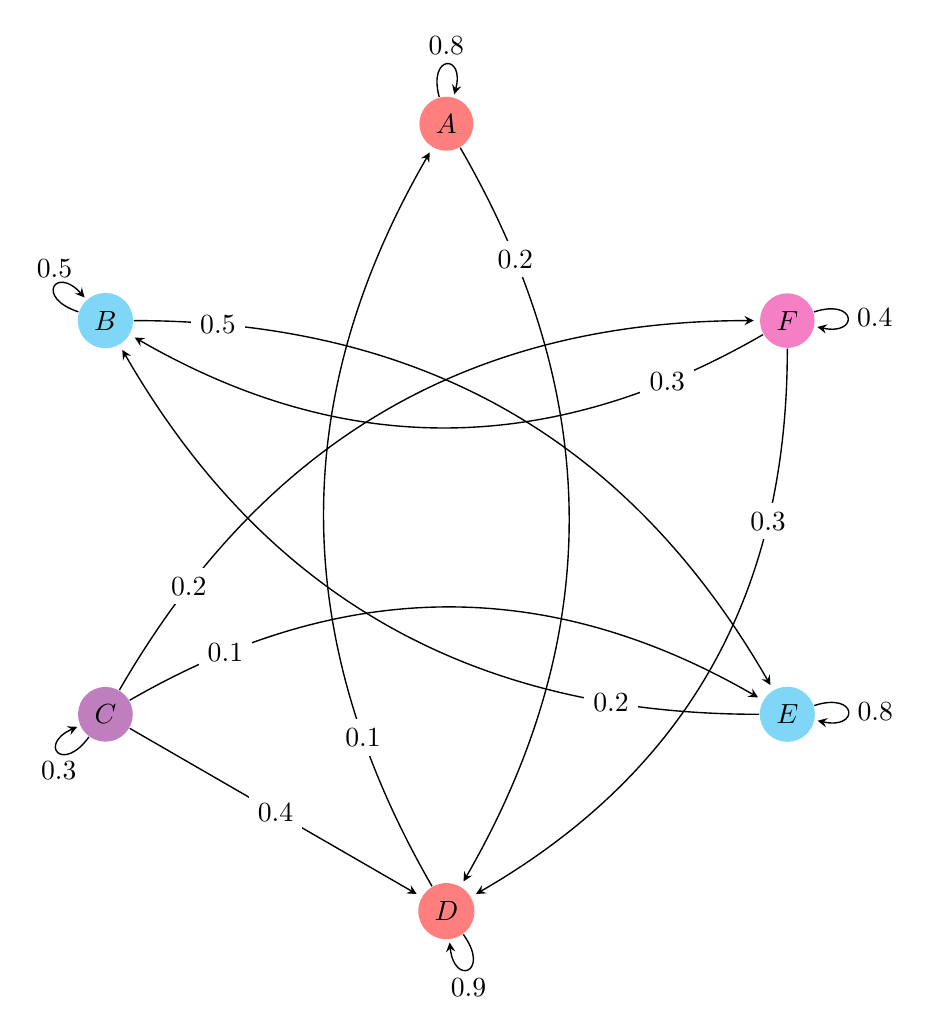
\begin{tikzpicture}[->,>=stealth,shorten >=2pt, line width=0.5pt, node distance=2cm]
% Nodos
\node [circle , fill=red, opacity=0.5,text opacity=1, text=black] (A)  at  (90:5cm) {$A$};
\node [circle , fill=cyan, opacity=0.5,text opacity=1, text=black] (B)  at (150:5cm) {$B$};
\node [circle , fill=violet, opacity=0.5,text opacity=1, text=black] (C)  at (210:5cm) {$C$};
\node [circle , fill=red, opacity=0.5,text opacity=1, text=black] (D)  at (270:5cm) {$D$};
\node [circle , fill=cyan, opacity=0.5,text opacity=1, text=black] (E)  at (330:5cm) {$E$};
\node [circle , fill=magenta, opacity=0.5,text opacity=1, text=black] (F)  at  (30:5cm) {$F$};
% Ejes
% ---
% A
% ---
\path (A) edge [loop above] node [above] {$0.8$} (A);

%\path (A) edge [bend left] node [fill=white, anchor=center, pos=0.3] {$0.3$} (B);

%\path (A) edge [bend left] node [fill=white, anchor=center, pos=0.7] {$0.3$} (C);

\path (A) edge [bend left] node [fill=white, anchor=center, pos=0.15] {$0.2$} (D);

%\path (A) edge [bend left] node [fill=white, anchor=center, pos=0.2] {$0.5$} (E);

%\path (A) edge [bend left] node [above right] {$0.5$} (F);

% ---
% B
% ---
\path (B) edge [in=132, out=162, loop] node [above] {$0.5$} (B);

%\path (B) edge [bend left] node [fill=white, anchor=center, pos=0.5] {$0.1$} (A);

%\path (B) edge [bend left] node [fill=white, anchor=center, pos=0.25] {$0.2$} (C);

%\path (B) edge [bend left] node [fill=white, anchor=center, pos=0.75] {$0.2$} (D);

\path (B) edge [bend left] node [fill=white, anchor=center, pos=0.1] {$0.5$} (E);

%\path (B) edge [bend left] node [fill=white, anchor=center, pos=0.7] {$0.5$} (F);
% ---
% C
% ---
\path (C) edge [in=204, out=234, loop] node [below] {$0.3$} (C);

%\path (C) edge [bend left] node [fill=white, anchor=center, pos=0.15] {$0.5$} (A);

%\path (C) edge [bend left] node [fill=white, anchor=center, pos=0.7] {$0.1$} (B);

\path (C) edge [] node [fill=white, anchor=center, pos=0.5] {$0.4$} (D);

\path (C) edge [bend left] node [fill=white, anchor=center, pos=0.15] {$0.1$} (E);

\path (C) edge [bend left] node [fill=white, anchor=center, pos=0.15] {$0.2$} (F);
% ---
% D
% ---
\path (D) edge [in=276, out=306, loop] node [below] {$0.9$} (D);

\path (D) edge [bend left] node [fill=white, anchor=center, pos=0.2] {$0.1$} (A);

%\path (D) edge [bend left] node [fill=white, anchor=center, pos=0.25] {$0.5$} (B);

%\path (D) edge [bend left] node [right] {$0.0$} (C);

%\path (D) edge [bend left] node [above right] {$0.0$} (E);

%\path (D) edge [bend left] node [fill=white, anchor=center, pos=0.7] {$0.6$} (F);
% ---
% E
% ---
\path (E) edge [in=348, out=18, loop] node [right] {$0.8$} (E);
%\path (E) edge [bend left] node [below] {$0.3$} (A);

\path (E) edge [bend left] node [fill=white, anchor=center, pos=0.18] {$0.2$} (B);

%\path (E) edge [bend left] node [right] {$0.0$} (C);

%\path (E) edge [bend left] node [fill=white, anchor=center, pos=0.5] {$0.4$} (D);

%\path (E) edge [bend left] node [fill=white, anchor=center, pos=0.5] {$0.6$} (F);
% ---
% F
% ---
\path (F) edge [in=348, out=18, loop] node [right] {$0.4$} (F);
%\path (E) edge [bend left] node [below] {$0.3$} (A);

\path (F) edge [bend left] node [fill=white, anchor=center, pos=0.15] {$0.3$} (B);

%\path (F) edge [bend left] node [right] {$0.0$} (C);

\path (F) edge [bend left] node [fill=white, anchor=center, pos=0.25] {$0.3$} (D);

%\path (F) edge [bend left] node [fill=white, anchor=center, pos=0.5] {$0.5$} (E);
\end{tikzpicture} 
\caption{Ejercicio 1d} 
\label{fig:1d}
\end{figure}
\begin{figure}[!hbt]
\centering
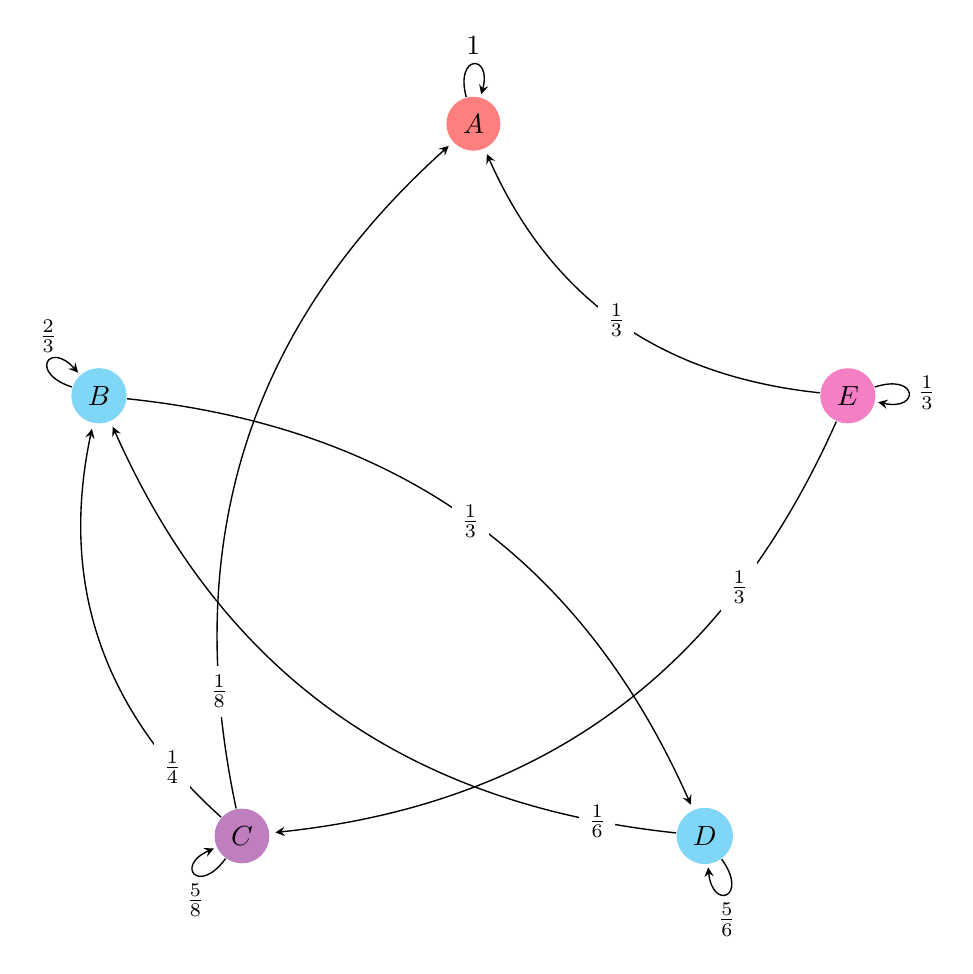
\begin{tikzpicture}[->,>=stealth,shorten >=2pt, line width=0.5pt, node distance=2cm]
% Nodos
\node [circle , fill=red, opacity=0.5,text opacity=1, text=black] (A)  at  (90:5cm) {$A$};
\node [circle , fill=cyan, opacity=0.5,text opacity=1, text=black] (B)  at (162:5cm) {$B$};
\node [circle , fill=violet, opacity=0.5,text opacity=1, text=black] (C)  at (234:5cm) {$C$};
\node [circle , fill=cyan, opacity=0.5,text opacity=1, text=black] (D)  at (306:5cm) {$D$};
\node [circle , fill=magenta, opacity=0.5,text opacity=1, text=black] (E)  at  (18:5cm) {$E$};
% Ejes
% ---
% A
% ---
\path (A) edge [loop above] node [above] {$1$} (A);

%\path (A) edge [bend left] node [fill=white, anchor=center, pos=0.3] {$0.3$} (B);

%\path (A) edge [bend left] node [fill=white, anchor=center, pos=0.7] {$0.3$} (C);

%\path (A) edge [bend left] node [right] {$0.0$} (D);

%\path (A) edge [bend left] node [fill=white, anchor=center, pos=0.5] {$1.0$} (E);

% ---
% B
% ---
\path (B) edge [in=132, out=162, loop] node [above] {$\frac{2}{3}$} (B);

%\path (B) edge [bend left] node [below] {$0.3$} (A);

%\path (B) edge [bend left] node [right] {$0.3$} (C);

\path (B) edge [bend left] node [fill=white, anchor=center, pos=0.5] {$\frac{1}{3}$} (D);

%\path (B) edge [bend left] node [above right] {$0.0$} (E);
% ---
% C
% ---
\path (C) edge [in=204, out=234, loop] node [below] {$\frac{5}{8}$} (C);

\path (C) edge [bend left] node [fill=white, anchor=center, pos=0.15] {$\frac{1}{8}$} (A);

\path (C) edge [bend left] node [fill=white, anchor=center, pos=0.15] {$\frac{1}{4}$} (B);

%\path (C) edge [bend left] node [fill=white, anchor=center, pos=0.15] {$0.3$} (D);

%\path (C) edge [bend left] node [above right] {$0.0$} (E);
% ---
% D
% ---
\path (D) edge [in=276, out=306, loop] node [below] {$\frac{5}{6}$} (D);

%\path (D) edge [bend left] node [below] {$0.3$} (A);

\path (D) edge [bend left] node [fill=white, anchor=center, pos=0.1] {$\frac{1}{6}$} (B);

%\path (D) edge [bend left] node [right] {$0.0$} (C);

%\path (D) edge [bend left] node [above right] {$0.0$} (E);
% ---
% E
% ---
\path (E) edge [in=348, out=378, loop] node [right] {$\frac{1}{3}$} (E);

\path (E) edge [bend left] node [fill=white, anchor=center, pos=0.5] {$\frac{1}{3}$} (A);

%\path (E) edge [bend left] node [fill=white, anchor=center, pos=0.25] {$0.3$} (B);

\path (E) edge [bend left] node [fill=white, anchor=center, pos=0.25] {$\frac{1}{3}$} (C);

%\path (E) edge [bend left] node [fill=white, anchor=center, pos=0.5] {$0.4$} (D);
\end{tikzpicture} 
\caption{Ejercicio 1e} 
\label{fig:1e}
\end{figure}